% Intended LaTeX compiler: pdflatex
\documentclass[10pt,a4paper,UTF8]{article}
\usepackage{zclorg}

\title{规范正交基}
\hypersetup{
 pdfauthor={},
 pdftitle={规范正交基},
 pdfkeywords={},
 pdfsubject={},
 pdfcreator={Emacs 25.0.50.1 (Org mode 9.0.5)},
 pdflang={English}}
\begin{document}

{\heiti\large \maketitle }
\tableofcontents
\titlepic{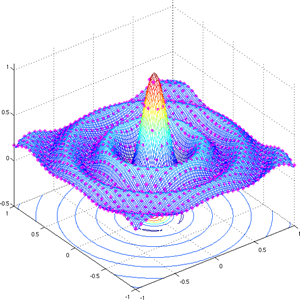
\includegraphics[scale=0.25]{../../img/sinc.PNG}}

\section{规范正交基}
\label{sec:org4a7389a}


\begin{definition}
如果一个向量组中每个向量的范数都是\(1\)且与其他向量正交,则称这个向量组是规范正交的。也就是说,\(V\)上的向量组\(e_{1},\ldots ,e_{n}\)是规范正交的,如果:
\begin{equation}
\label{eq:1}
\langle e_{j},e_{k} \rangle =
\begin{cases}
1 & j = k \\
0 & j\neq k
\end{cases}
\end{equation}
\end{definition}
\begin{instance}
\begin{enumerate}
\item \(\mathbf{F}^{n}\)的标准基是规范正交组
\item \((\frac{1}{\sqrt{3}},\frac{1}{\sqrt{3}} ,\frac{1}{\sqrt{3}})\) \((-\frac{1}{\sqrt{2}},-\frac{1}{\sqrt{2}} ,0)\) 是\(\mathbf{F}^{3}\)的规范正交组
\item \((\frac{1}{\sqrt{3}},\frac{1}{\sqrt{3}} ,\frac{1}{\sqrt{3}})\) \((-\frac{1}{\sqrt{2}},-\frac{1}{\sqrt{2}} ,0)\), \((\frac{1}{\sqrt{6}}, \frac{1}{\sqrt{6}}, -\frac{2}{\sqrt{6}})\) 是\(\mathbf{F}^{3}\)的规范正交组.
\end{enumerate}
\end{instance}

规范正交线性组合的范数:

若\(e_{1},\ldots ,e_{m}\)是\(V\)中的规范正交向量组,则对所有的\(a_{1},\ldots ,a_{m}\in \mathbf{F}\)均有:
\begin{equation}
\label{eq:2}
\| a_{1}e_{1} + \ldots + a_{m}e_{m} \|^{2} = |a_{1}|^{2} + \ldots + |a_{m}|^{2}
\end{equation}

\begin{theorem}
每个规范正交向量组都是线性无关的
\end{theorem}
\begin{proof}
设\(e_{1},\ldots ,e_{m}\)是一组规范正交向量组,并设\(a_{1},\ldots ,a_{m}\in \mathbf{F}\),使得:
\begin{equation}
\label{eq:3}
a_{1}e_{1} + \ldots a_{m}e_{m} = 0
\end{equation}
所以有\(|a_{1}|^{2} + \ldots |a_{m}|^{2} = 0\),所以\(a_{1} = \ldots = a_{m} = 0\)
\end{proof}

\begin{definition}
\(V\)的规范正交基是\(V\)中的规范正交向量组成的基。\(V\)中的每个长度为\(\dim V\)的规范正交向量组都是\(V\)的规范正交基。
\end{definition}
一般的,给定\(V\)的规范正交基\(e_{1},\ldots ,e_{n}\)和向量\(v\in V\),存在标量\(a_{1},\ldots ,a_{n}\)使得:
\[v= a_{1}e_{1} + \ldots + a_{n}e_{n}\]

我们可以把向量写成规范正交基的线性组合。设\(e_{1},\ldots ,e_{n}\)是\(V\)的规范正交基,且\(v\in V\),则:
\begin{equation}
\label{eq:4}
v= \langle v,e_{1} \rangle e_{1} + \ldots \langle v,e_{n} \rangle e_{n}
\end{equation}
且:
\begin{equation}
\label{eq:5}
\| v \|^{2} = | \langle v,e_{1} \rangle  |^{2} + \ldots + | \langle v,e_{n} \rangle  |^{2}
\end{equation}

\section{格拉姆-施密特过程}
\label{sec:org45c8eb9}


规范正交基有这么好的作用,那么如何找到这个规范正交基呢?格拉姆-施密特过程可以把一个线性无关组转化成与原来的组有相同张成空间的规范正交基。

\begin{theorem}
设\(v_{1},\ldots ,v_{m}\)是\(V\)的线性无关向量组。设\(e_{1} = \frac{v_{1}}{\| v_{1} \| }\),对于\(j = 2,\ldots ,m\)定义\(e_{j}\)如下:
\begin{equation}
\label{eq:6}
e_{j} = \frac{v_{j} - \langle v_{j},e_{1} \rangle e_{1} - \ldots - \langle v_{j},e_{j-1} \rangle e_{j-1}   }{ \| v_{j} - \langle v_{j},e_{1} \rangle e_{1} - \ldots - \langle v_{j},e_{j-1} \rangle e_{j-1}  \| }
\end{equation}
则\(e_{1},\ldots ,e_{m}\)是\(V\)中的规范正交组,使得对\(j=1,\ldots ,m\)都有:
\begin{equation}
\label{eq:7}
\mathrm{span}(v_{1},\ldots ,v_{j}) = \mathrm{span}(e_{1},\ldots ,e_{j})
\end{equation}
\end{theorem}

\begin{proof}
我们将对\(j\)用归纳法来证明结论成立。首先\(j=1\)时,由\(v_{1}\)是\(e_{1}\)的正数倍所以\[ \mathrm{span} (v_{1}) = \mathrm{span}(e_{1})\]

设\(1 < j < m\)并假设已经有:
\[ \mathrm{span}(v_{1},\ldots ,v_{j-1})  = \mathrm{span}(e_{1},\ldots ,e_{j-1})\]
注意\(v_{j}\notin \mathrm{span}(v_{1},\ldots ,v_{j-1})\),因为\(v_{1},\ldots ,v_{m}\)是线性无关的。于是\(v_{j}\notin \mathrm{span}(e_{1},\ldots ,e_{j-1})\) 因此有\(\| e_{j} \| = 1\)。

设\(1 \leq k < j\)则:
\begin{eqnarray}
\label{eq:9}
\langle e_{j},e_{k} \rangle  &=&  \bigg \langle \frac{v_{j} - \langle v_{j},e_{1} \rangle e_{1} - \ldots - \langle v_{j},e_{j-1} \rangle e_{j-1}   }{ \| v_{j} - \langle v_{j},e_{1} \rangle e_{1} - \ldots - \langle v_{j},e_{j-1} \rangle e_{j-1} \|} ,e_{k} \bigg\rangle \\
&=&\frac{ \langle v,e_{k} \rangle - \langle v,e_{k} \rangle   }{  \| v_{j} - \langle v_{j},e_{1} \rangle e_{1} - \ldots - \langle v_{j},e_{j-1} \rangle e_{j-1} \|} \\
&=& 0
\end{eqnarray}
因此\(e_{1},\ldots ,e_{j}\)是规范正交组。
\end{proof}

\begin{instance}
求\(\mathcal{P}_{2}(\mathbf{R})\)的一个规范正交基,这里的内积为\((p,q)= \int_{-1}^{1}p(x)q(x)dx\)
我们知道\(\mathcal{P}_{2}(\mathbf{R})\)的一个基为\(1,x,x^{2}\),现在对这个基执行格拉姆施密特过程。

首先对于\(v_{1} = 1\),我们有:
\begin{eqnarray}
\label{eq:8}
e_{1}&=& \frac{v_{1}}{ \| v_{1} \| } \\
&=& \frac{1}{ \sqrt{\int_{-1}^{1} 1 dx }} \\
&=& \frac{1}{\sqrt{2}}
\end{eqnarray}

对于\(e_{2}\),我们首先计算格拉姆施密特过程的分子部分:
\begin{eqnarray}
\label{eq:10}
v_{2} - \langle v_{2},e_{1} \rangle e_{1}  &=& x - \int_{-1}^{1} x\frac{1}{\sqrt{2}}dx \frac{1}{\sqrt{2}} \\
&=& x
\end{eqnarray}
然后计算分子部分:
\begin{eqnarray}
\label{eq:11}
\| v_{2} -  \langle v_{2},e_{1} \rangle e_{1}  \| &=& \sqrt{ \int_{-1}^{1} x^{2} dx  } \\
&=& \sqrt{\frac{2}{3}}
\end{eqnarray}
所以:
\begin{equation}
\label{eq:12}
e_{2} = \sqrt{ \frac{3}{2}} x
\end{equation}
对于\(e_{3}\),先求得分子部分:
\begin{eqnarray}
\label{eq:13}
x^{2} &-& \langle x^{2},e_{1} \rangle e_{1} - \langle x^{2},e_{2} \rangle e_{2}  \\
&=& x^{2} - \int_{-1}^{1}x^{2}\sqrt{\frac{1}{2}}dx \frac{1}{\sqrt{2}} - \int_{1}^{1}x^{2}\sqrt{\frac{3}{2}}x dx \sqrt{\frac{3}{2}}x = x^{2} - \frac{1}{3}
\end{eqnarray}
对于分母部分:
\begin{eqnarray}
\label{eq:14}
\| x^{2} - \frac{1}{3} \|^{2} &=& \int_{-1}^{{1}} (x^{2} - \frac{1}{3})^{2}dx \\
&=& \frac{8}{45}
\end{eqnarray}
所以\[\| x^{2} - \frac{1}{3} \|  = \sqrt{\frac{8}{45}}\]
进而\(e_{3} = \sqrt{\frac{45}{8}} (x^{2} - \frac{1}{3})\)
\end{instance}

\begin{theorem}
每个有限维内积空间都有规范正交基
\end{theorem}

\begin{proof}
设\(V\)是有限维的,取\(V\)的一个基,对他应用格拉姆施密特过程,则得到一个\(\dim V\)的规范正交组,这个规范正交组就是\(V\)的规范正交基。
\end{proof}

不仅规范正交基是存在的,而且任何规范正交组都可以扩展为规范正交基。
\begin{theorem}
设\(T\in \mathcal{L}(V)\),如果\(T\)关于\(V\)的某个基具有上三角矩阵,那么\(T\)关于\(V\)的某个规范正交基也具有上三角矩阵。
\end{theorem}

\begin{proof}
设\(T\)关于\(V\)的基\(v_{1},\ldots ,v_{n}\)具有上三角矩阵,则对每个\(j = 1,\ldots ,n\)均有\(\mathrm{span}(v_{1},\ldots ,v_{n})\)

对\(v_{1},\ldots ,v_{n}\)应用格拉姆施密特过程,得到\(V\)的规范正交基\(e_{1},\ldots ,e_{n}\),因为对每个\(j\)都有:
\[ \mathrm{span}(e_{1},\ldots ,e_{j} ) = \mathrm{span}(v_{1},\ldots ,v_{j}) \]
所以对每个\(j=1,\ldots ,n\)均有\(\mathrm{span}(e_{1},\ldots ,e_{j})\)在\(T\)下不变。因此,\(T\)关于规范正交基\(e_{1},\ldots ,e_{n}\)有上三角矩阵。
\end{proof}

\begin{theorem}
\textbf{舒尔定理} 设\(V\)是有限维的复向量空间且\(T\in \mathcal{L}(V)\),则\(T\)关于\(V\)的某个规范正交基具有上三角矩阵。
\end{theorem}

\section{内积空间上的线性泛函}
\label{sec:org749f839}


\begin{definition}
\(V\)上的线性泛函是从\(V\)到\(\mathbf{F}\)的线性映射。也就是说,线性泛函是\(\mathcal{L}(V, \mathbf{F})\)中的元素。
\end{definition}
\begin{instance}
如下定义的函数\(\varphi : \mathbf{F}^{3} \rightarrow \mathbf{F}\)
\[\varphi(z_{1},z_{2},z_{3}) = 2z_{1} - 5z_{2} + z_{3}\]是\(\mathbf{F}^{3}\)上的线性泛函。我们可以将这个线性泛函写成如下的形式:对每个\(z\in \mathbf{F}^{3}\) \[\varphi(z) = \langle z,u \rangle  \]
其中\(u = (2,-5,1)\)
\end{instance}
\begin{instance}
如下定义的函数\(\varphi : \mathcal{P}_{2}(\mathbf{R}) \rightarrow \mathbf{R}\) \[ \varphi(p) = \int_{-1}^{1} p(t)\cos(\pi t)dt \]是\(\mathcal{P}_{2}(\mathbf{R})\)上的线性泛函。这里\(\mathcal{P}_{2}(\mathbf{R})\)上的内积是\([-1,1]\)上的两个函数相乘后做定积分。存在\(u\in \mathbf{P}_{2}(\mathbf{R})\)使得对任意\(p\in \mathcal{P}_{2}(\mathbf{R})\)均有:\[\varphi(p) = \langle p,u \rangle  \] 我们不能取\(u(t) = \cos(\pi t)\),因为它不是\(\mathcal{P}_{2}(\mathbf{R})\)中的元素。
\end{instance}

如果\(u\in V\)那么把\(v\)映射成\(\langle v,u \rangle\)的映射是\(V\)上的线性泛函。下述定理表明,\(V\)上的每个线性泛函都是这种形式。
\begin{theorem}
\textbf{里斯表示定理} 设\(V\)是有限维的且\(\varphi\)是\(V\)上的线性泛函,则存在唯一的向量\(u\in V\)使得对每个\(v\in V\)均有\(\varphi(v)= \langle v,u \rangle\)
\end{theorem}

\begin{proof}
先证明存在向量\(u\in V\)使得对每个\(v\in U\)均有\(\varphi(v)= \langle v,u \rangle\), 设\(e_{1},\ldots ,e_{n}\)是\(V\)的规范正交基,则对每个\(v\in V\)均有:
\begin{eqnarray}
\label{eq:15}
\varphi(v)&=& \varphi ( \langle v,e_{1} \rangle e_{1} + \ldots + \langle v,e_{n} \rangle e_{n}   ) \\
&=& \langle v,e_{1} \rangle \varphi(e_{1}) + \ldots + \langle v,e_{n} \rangle \varphi(e_{n}) \\
&=& \langle v, \overline{\varphi(e_{1})}e_{1} \rangle  + \ldots + \langle v,\overline{\varphi(e_{n})}e_{n} \rangle \\
&=& \langle v, \overline{\varphi(e_{1})}e_{1} + \ldots + \overline{\varphi(e_{n})}e_{n} \rangle
\end{eqnarray}
令\(u = \overline{\varphi(e_{1})}e_{1} + \ldots + \overline{\varphi(e_{n})}e_{n}\),因此,有:
\[\forall v\in V, \varphi(v) = \langle v,u \rangle  \]
现在来证明只有一个向量\(u\in V\)满足条件。设\(u_{1},u_{2}\in V\)使得对每个\(v\in V\)均有:
\[\varphi(v) = \langle v,u_{1} \rangle  = \langle v,u_{2} \rangle  \]
则对每个\(v\in V\)均有:
\[0 = \langle v,u_{1} \rangle - \langle v,u_{2} \rangle = \langle v,u_{1}-u_{2} \rangle   \]
令\(v = u_{1} - u_{2}\),则有\(u_{1} - u_{2} = 0\),即\(u_{1} = u_{2}\)这就完成了唯一性证明。
\end{proof}

\begin{instance}
求\(u\in \mathcal{P}_{2}(\mathbf{R})\)使得对每个\(p\in \mathcal{P}_{2}(\mathbf{R})\)均有:
\[\int_{-1}^{1} p(t)(\cos(\pi t)) dt = \int_{-1}^{1} p(t)u(t)dt\]
\textbf{解} 设\(\varphi(p) = \int_{-1}^{1} p(t)\cos(\pi t)dt\),则:
\begin{eqnarray}
\label{eq:16}
u(x)&=& \int_{-1}^{1} \frac{1}{\sqrt{2}} (\cos(\pi t))  dt \frac{1}{\sqrt{2}} \\
&+&\int_{-1}^{1} \sqrt{\frac{3}{2}} t (\cos(\pi t))  dt \sqrt{\frac{3}{2}} x \\
&+&\int_{-1}^{1} \sqrt{\frac{45}{8}} (t^{2} - \frac{1}{3}) (\cos(\pi t))  dt \sqrt{\frac{45}{8}} (x^{2} - \frac{1}{3})
\end{eqnarray}
计算可得:
\[u(x) = -\frac{45}{2\pi^{2}}(x^2 - \frac{1}{3})\]
\end{instance}

设\(V\)是有限维的且\(\varphi\)是\(V\)上的线性泛函,则
\[u = \overline{\varphi(e_{1})}e_{1} + \ldots + \overline{\varphi(e_{n})} e_{n}\]
给出了对所有\(v\in V\)均有\(\varphi(v) = \langle v,u \rangle\)。看起来右端依赖于规范正交基\(e_{1},\ldots ,e_{n}\)和\(\varphi\),然而里斯表示定理告诉我们\(u\)是由\(\varphi\)唯一确定的。所以等式右端与\(V\)的规范正交基\(e_{1},\ldots ,e_{n}\)的选取无关。
\end{document}
